\iffalse
\documentclass[12pt]{article}
\usepackage{graphicx}
\usepackage[none]{hyphenat}
\usepackage{graphicx}
\usepackage{listings}
\usepackage[english]{babel}
\usepackage{graphicx}
\usepackage{caption} 
\usepackage{booktabs}
\usepackage{array}
\usepackage{amssymb} % for \because
\usepackage{amsmath}   % for having text in math mode
\usepackage{extarrows} % for Row operations arrows
\usepackage{listings}
\lstset{
  frame=single,
  breaklines=true
}
\usepackage{hyperref}
  
%Following 2 lines were added to remove the blank page at the beginning
\usepackage{atbegshi}% http://ctan.org/pkg/atbegshi
\AtBeginDocument{\AtBeginShipoutNext{\AtBeginShipoutDiscard}}


%New macro definitions
\newcommand{\mydet}[1]{\ensuremath{\begin{vmatrix}#1\end{vmatrix}}}
\providecommand{\brak}[1]{\ensuremath{\left(#1\right)}}
\providecommand{\norm}[1]{\left\lVert#1\right\rVert}
\newcommand{\solution}{\noindent \textbf{Solution: }}
\newcommand{\myvec}[1]{\ensuremath{\begin{pmatrix}#1\end{pmatrix}}}
\providecommand{\abs}[1]{\left\vert#1\right\vert}
\let\vec\mathbf

\begin{document}

\begin{center}
\title{\textbf{Equation  of Perpendicular}}
\date{\vspace{-5ex}} %Not to print date automatically
\maketitle
\end{center}
\setcounter{page}{1}
\section{12$^{th}$ Maths - Chapter 11}
\textbf{This is Problem-2 from Exercise 11.2}
\begin{enumerate}
\item Show that the line through the points (1, -1, 2), (3, 4, -2) is perpendicular to the line through the points (0, 3, 2) and (3, 5, 6).
\item \textbf{Solution :}
	\fi
	Let
\begin{align}  
\vec{A}=\myvec{1 \\-1\\2},\,
\vec{B}=\myvec{3 \\ 4\\-2},\,
\vec{C}=\myvec{0 \\ 3\\2},\,
\vec{D}=\myvec{3 \\ 5\\6}.
\end{align}
Then
\begin{align}
\vec{A}-\vec{B} &= \brak{\myvec{1 \\-1\\ 2 } - \myvec{3 \\4\\-2 } } = \myvec{2 \\ 5\\-4 }\\
\vec{C}-\vec{D} &= \brak{\myvec{0 \\ 3\\2 } - \myvec{3 \\5\\6} } = \myvec{3\\2\\4}\\
\implies 
	\brak{\vec{A}-\vec{B} }^{\top}
	\vec{C}-\vec{D} &=
 \myvec{2 & 5& -4}\myvec{3 \\2\\4 } = \vec{0}
\end{align}
Thus, 
$AB\perp CD$.

%\begin{figure}[h!]
%	  \centering 
%	  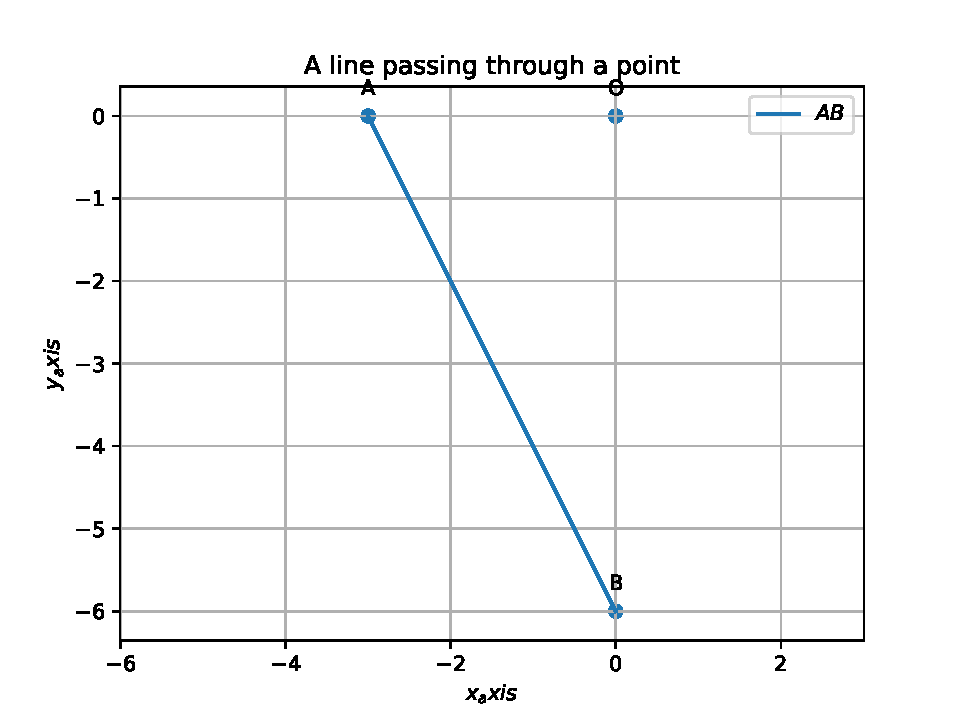
\includegraphics[width=\columnwidth]{line1.pdf}
%	  \caption{}
%	  \label{fig:line1.pdf}
%	  \end{figure} 	 		  

